\documentclass[]{article}
\setlength{\parskip=0.7}{\baselineskip}
\setlength{\parindent}{0pt}

\usepackage{times}
\usepackage{fullpage}

\usepackage{epsfig}
\usepackage{subfigure}

\usepackage{listings}
\usepackage{siunitx}
\usepackage[super]{nth}

\usepackage[sharp]{easylist}

\usepackage[table,xcdraw]{xcolor}

\definecolor{NavyBlue}{cmyk}{0.94,0.54,0,0.5}
\definecolor{BrickRed}{cmyk}{0.16,0.89,0.61,0.2}
\usepackage{url}
\usepackage{breakurl}

\usepackage[
        colorlinks=true,
        urlcolor=NavyBlue, 
        linkcolor=NavyBlue, 
        bookmarksopen=true]{hyperref}
\hypersetup{
    colorlinks,citecolor=NavyBlue,
    linkcolor={red!50!black},
    urlcolor={blue!90!black}
}


\newcommand{\us}{$\mu$s }
\newcommand{\subtopic}[1]{\vspace{1.5pt} \noindent \textbf{#1}}

\definecolor{notecolor}{rgb}{0.75,0,0} % A darker red
\definecolor{hlcolor}{RGB}{0,0,205}
\newcommand{\todo}[1]{\textcolor{notecolor}{\textbf{TODO: #1}}}
\newcommand{\hl}[1]{\textcolor{hlcolor}{#1}}
\newcommand{\fixit}[2][]{\textcolor{notecolor}{%
     \ifthenelse{\isempty{#1}}{\textbf{[Fixit: %
         #2]}}{\textbf{#2\footnote{\textcolor{notecolor}{Fixit: #1}}}}}}
\newenvironment{highlight}{\par\color{notecolor}}{\par}





\begin{document}

\title{Kawkab: A Distributed Filesystem for Fast Data}
%\author{Sajjad Rizvi, Bernard Wong}
\date{}
\maketitle

\bgroup
\def\arraystretch{1.5}
\begin{table}[!htb]
\centering
\caption{Change Log}
\label{table:change-log}
\begin{tabular}{|l|l|l|}
\hline
\rowcolor[HTML]{EFEFEF} 
Date             & Description  & Participants  \\ \hline
 August 03, 2017  & Kawkab single node design: TBD      & Sajjad  \\ \hline
 March 03, 2017  & Kawkab single node design           & Sajjad  \\ \hline
 March 10, 2017  & - Added sections 3 and 4, about the distributed design of Kawkab& \\ 
                 & - Updated architecture diagram & Sajjad  \\ \hline
\end{tabular}
\end{table}
\egroup


\section{Introduction} 

Kawkab is a distributed filsesystem developed to efficiently manage large
amounts of streaming data. Unlike traditional filesystem that are designed for
bulk data transfers in the context of Big Data, Kawkab manages the storage for
fast streaming data with the focus on memory management, read/write
performance, and scalability.


Kawkab's design is mainly motivated from the design approach of a standard Unix filesystem.
However, unlike a disk-based traditional filesystem, Kawkab is an append only
system  and the location of the blocks is not fixed to a specific storage
medium. Kawkab assumes the availability of an extensible backend storage that
can store large volumes of data. Unlike other distributed filesystems such
as Tachyon, Kawkab enables reading most recent data of the files even if the
last block of the file is not full and sealed. 
%The reasons to follow the Unix filesystem is to control the memory usage of the
%system and make the system memory efficient.

Kawkab is designed for the single writer and multiple readers use case. Kawkab
allows only one node at a time to perform file append operations. Moreover,
the file appender is restricted to be a distinguished node that created
the file. Other nodes can only read the files.




\section{Architecture} 

\begin{figure}[t]
    \centering
    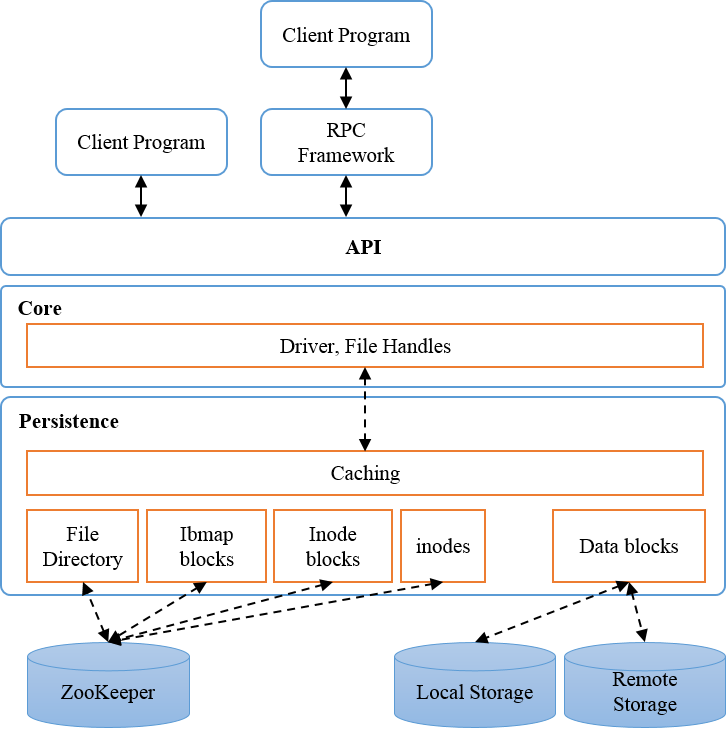
\includegraphics[width=0.55\columnwidth]{{figures/architecture.png}}
    \caption{Kawkab architecture.}
   \label{fig:architecture}
\end{figure}


\begin{figure}[t]
    \centering
    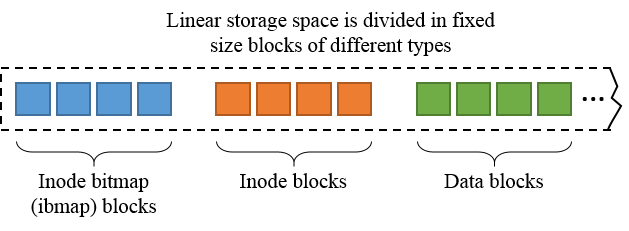
\includegraphics[width=0.5\columnwidth]{{figures/linear-space.png}}
    \caption{Filesystem is designed as a very large storage space organized in fixed size blocks.}
   \label{fig:storage-space}
\end{figure}

\begin{figure}[t]
    \centering
    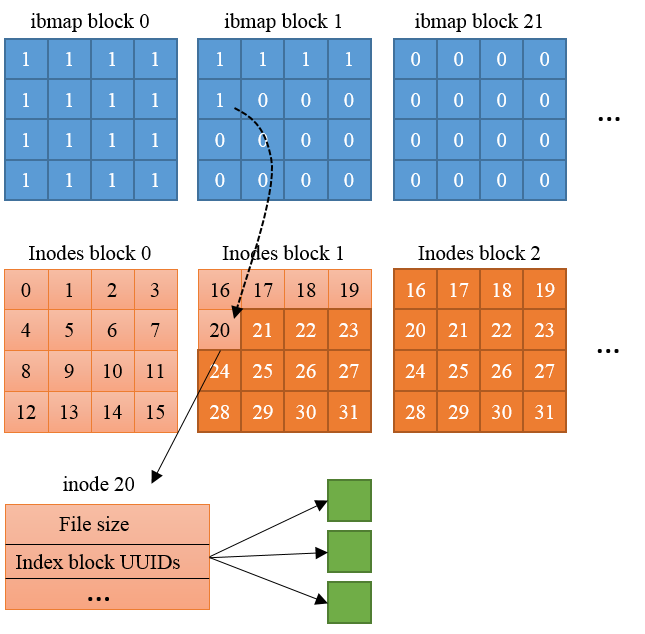
\includegraphics[width=0.5\columnwidth]{{figures/blocks-layout.png}}
    \caption{Relationship between different types of blocks.}
   \label{fig:blocks-layout}
\end{figure}


\begin{figure}[t]
    \centering
    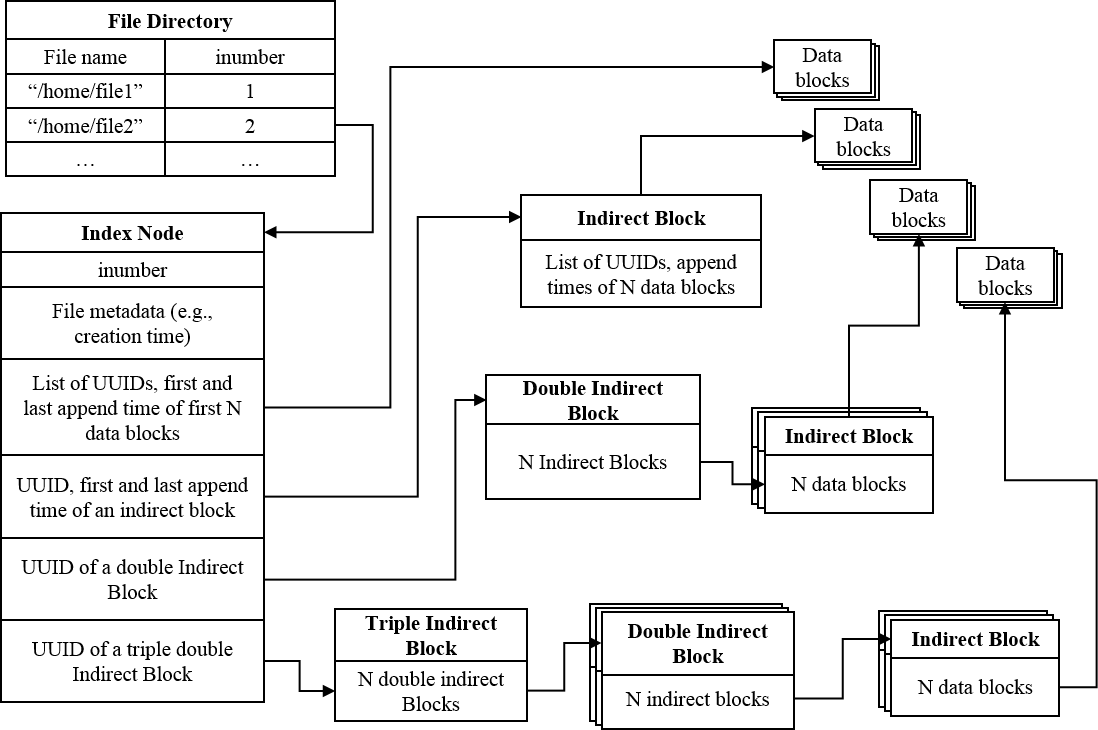
\includegraphics[width=0.7\columnwidth]{{figures/file-index-design.png}}
    \caption{File directory and file index.}
   \label{fig:data-structures}
\end{figure}




At the high level, the system consists of four fixed size structures: a file directory,
inode-bitmap blocks, inode blocks, and data blocks.


\subsection{Namespace and File Directory}
A file consists of metadata and fixed size data blocks that are persistently
stored in an extensible storage such as Amazon S3 or Dynamo.
Each file has a unique fully qualified name, which a client assigns when the client
creates the file. The clients access the files using the filenames.
However, internally, Kawkab assigns a globally unique 64-bit number to each file, which is
called \textit{inumber}. Internally the files are referred through 
their inumbers. The filename to inumber mappings are stored in the \textit{file directory},
which is explained in the next section.

Kawkab does not support directory hierarchies. Instead, all the files are stored
as a flat storage system. However, the filenames can be qualified to represent
directories, e.g., ``/home/smash/file''.

\subtopic{File Directory:}
In our current design, the file directory is implemented as a distributed
key-value store, where the keys are the filenames and the values are the corresponding
inumbers. We propose to use ZooKeeper as the key-value store because of its
atomically \textit{zknode}-creation functionality that returns an error if
the \textit{zknode} already exists. However, any distributed key-value store can be used 
that provides atomic updates to the key-value store.


\subsection{Inode Bitmap Blocks}
A node keeps track of the assigned and available inumbers using an \textit{inodes-bitmap}.
Each node has a fixed size inodes-bitmap, which is divided in several sequential blocks
called \textit{ibmap-blocks}. Each bit in the bitmap translates to an index in the
\textit{inodes-block} structure, which is further explained below.
Figure~\ref{fig:blocks-layout} shows the relationship between the ibamap blocks, 
inode blocks, and the data blocks. Each bit at index $i$ in the
ibmap indicates whether inumber $i$ or the inode at index $i$ in the inode-blocks
is already used or not.

\subtopic{Inumber Assignment:}
A node linearly searches the ibmap-blocks to find the next unset bit in the ibmap.
To optimize the search, the node starts searching from the last position it
found the unused bit. When a file is deleted, which we expect to be extremely
rare, the bit is unset in the ibmap.


%An inode bitmap block, or ibmap block, is a
%fixed size block that contains part of the ibmap.  
%When a new file is created, Kawkab scans the ibmap to find the first unused 
%inumber and assigns that inumber to the inode associated with the file. Moreover,
%Kawkab sets the bit in the bitmap that is associated with the inumber.
%When a file is deleted, Kawkab clears the bit in the ibmap, which allows
%Kawkab to reuse the inode and the inumber for the next new file.

\subtopic{Metadata Sharding:} As the system consists of several nodes,
different nodes can concurrently create files that lead to inumber conflicts,
i.e., different nodes assigning same inumber to different files.  In order to
inumber conflicts and to  consistently maintain metadata without significant
communication overhead between the nodes, the 64-bit space of inumbers is
linearly sharded across the nodes. A node assigns a unique inumber to a new
file only from its own shard. This ensures that a node can assign an inumber
to a file without communicating over the network and without consensus
with the other nodes.

Sharding splits the 64-bit inumber space across all the nodes that may lead to
two concerns. First, a node may run out of the inumbers in its shard, which
will prevent the node from creating new files.  However, this is highly
unlikely due to the large size of shard assigned to each node. For example, if
the system is designed for $2^{20}$ nodes (1.04 million nodes), each nodes is
assigned nearly $2^{63} / 2^{20} = 2^{43} = 8.79 * 10^{12}$ inumbers, which is a
sufficiently large shard for a single node. If a node creates a new file
every 100 microseconds, i.e., $10000$ files per second, it will take almost
$39.7$ years to run out of the inumbers. In addition to the large shard
sizes, a node reuses the inumber when the file is deleted.

Second concern is about running out of inumber-shards. For example, if
the nodes fail and new nodes join enough number of times that exceed the maximum
number of nodes (1.04 million in the previous example), the system can run out
of inumbers globally. To prevent this situation, Kawkab allows reassigning
shards to other nodes. A new node can be assigned the shard of the previously
failed node.

%To prevent a node from running out of inumbers,
%the inumbers of the deleted files are reused.  Moreover, a failed node's shard
%can be reassigned to another node in order to prevent the filesystem from
%running out of the inumbers.  

\subtopic{Storing Sharding Information:}
The inumber sharding information is also stored in the key-value store, where the
keys are the node IDs and the values are the inumber-ranges assigned to the
nodes. The system ensures that the inumber-ranges assigned to different nodes
are disjoint. [TBD: How to ensure that the ranges are non-overlapping?]


%A virtual file comprises of metadata and data blocks.  The storage space is a
%collection of fixed size blocks $\{B_1, B_2, \ldots, B_N\}$.  Each block has a
%unique ID (UUID), and the blocks are persistently stored as files on the local
%storage devices (HDDs, SSDs) and the cloud, e.g., Amazon S3.
%
%The blocks in the storage space are of three types: index-node-bitmap blocks,
%index-node blocks, and data blocks.

\subsection{Inodes and Inode-blocks} 

Each node is assigned a fixed number of \textit{index-node blocks}
(\textit{inode blocks})  where an inode-block is a fixed size structure
consisting of fixed number of \textit{index-nodes} (\textit{inodes}).  An inode
is the main structure that keeps track of the file metadata that associates
data blocks with the files.


\subtopic{Inode:} Kawkab stores metadata of a file in a fixed size structure
called \textit{index node} or \textit{inode}. An inode is uniquely identified by
the \textit{inumber} assigned to the file with the inode is associated.

The metadata stored in an inode includes the current file size and other
information such as file creation time. Moreover, the inode includes
the IDs of the blocks that store the data-index of the file.
\hl{TBD: More about index storage when we add time series index in the
filesystem.}


%\hl{TODO: Update the following list to mention that the indirect blocks
%only contains the indices for the data, not the actual data blocks.
%The data blocks are identified and accessed using their IDs which
%is a combination of inumber and the block number.}
%
%\begin{enumerate}
%  \item \subtopic{File Metadata:} The file metadata consists of information
%        about the file such as file creation time, last access time, file
%        rights, and file size.
%
%	\item \subtopic{First $N$ Data Index Blocks:} An inode contains a fixed number
%$N$ of the IDs of the first $N$ data index blocks associated with the file.
%A data index block contains the indices of the data stored in the data blocks
%associated with the file.
%The number $N$ is kept small to optimize for the memory space and the file
%access for smaller files. 
%
%  \item \subtopic{Indirect Block:} 
%An inode contains the ID of one indirect block, where an indirect block is
%special data block that only consists of the IDs of the data blocks associated
%with the file. Thus, an indirect block is level-1 index into the file.
%As the size of each block is fixed, an indirect block contains the
%IDs of a fixed number of data blocks in a file. These data blocks 
%range from $N+1$ to $M$ where $M$ is the number of IDs stored in the
%direct block.
%
%  \item \subtopic{Double and Triple Indirect Block:}
%An inode has one double and one triple indirect block. A double indirect block is a two
%level index, i.e., a double indirect block is the ID of a special data block that contains
%the IDs of indirect blocks. Similarly, a triple indirect block contains the IDs of the
%double indirect blocks. These indexing levels are sufficient to support the maximum 
%file size in Kawkab, which is $2^{63}-1$ bytes.
%
%\end{enumerate}

\subtopic{Inode Blocks:} A collection of inodes are stored in a fixed size
structure called \textit{inode block}. An inode block consists of a fixed
number of a series of inodes. 


\subtopic{Locating an inode-block:} An inode-block is uniquely identified by
the inode-block number.  Because the inode-blocks are fixed size and contains a
fixed number of inodes, the block number can be easily calculated from the
inumber assigned to the file.
%, which is briefly described as follows.  As each inode has a fixed size $S_I$
%bytes, an inode block $B$ contains $N = S_{B} / S_I$ number of inodes, where
%$S_B$ is the size of an inodes block.  Thus, the inumber $x$ is located in the
%inode block number $ x / N$. In this way, given an inumber, Kawkab can
%calculate number of the inode block that contains the associated inode, and
%the index of the inode inside the block.
Figure~\ref{fig:blocks-layout} depicts the way ibmap, inode blocks, and the
inodes are related to each other.

%When a file is created, the file is assigned a unique inumber, which is the
%first available inode number in the system. To achieve that, the system keeps
%track of the inumbers already assigned using a bitmap called \textit{inode
%bitmap} or \textit{ibmap}. The ibmap is stored in the blocks of type "inode
%bitmap block".

%\subsection{Data Blocks} Kawkab has fixed size data blocks. Each data block has
%a unique ID, generated as a UUID.  Each block is persistently stored as a file
%in the persistent storage of the system, e.g., local or remote disks, EB3, or
%S3.  The name of the persistent file is extracted from the UUID: the UUID is
%converted to an ASCII character string using Base64 encoding.  The ASCII name
%is then converted into a file path such that each two characters in the ASCII
%representation of the UUID become a directory name in the persistent storage.
%For example, a UUID \texttt{ABCDEFGH} is stored as a file
%\texttt{/storage/datablocks/AB/CD/EF/GH}.


\subsection{Data blocks}

Data blocks contain the actual data belonging to the files in the system.
Each file is divided into fixed-size blocks that are stored persistently in
the global storage. Initially the blocks are created and filled with data
in the local storage. When the block is full, it is sealed and transferred 
to the global storage. 

All the files have same and fixed size of data blocks. Kawkab stores
individual data blocks as actual files in the underlying local storage and 
the global storage. Therefore, it is recommended that a larger block
size is used for local and global storage efficiency. 

\subtopic{Segments in Blocks:} Each data block is further partitioned into
fixed size segments for better memory management. For example, a 64MB data
block can be partitioned into 64 segments of size 1MB.  
%A block is not physically partitioned as segments on the local or global
%storage. Instead, a segment is just an abstraction for better memory
%management. 
The files are read in segments instead of blocks that reduces internal
fragmentation in memory.  During the file read and append operations, the cache
sub-system of Kawkab reserves memory for a segment instead of a block. As a
result, a large number of partially filled blocks do not waste a large portion
of memory.  For instance, if 1000 files are concurrently being appended, the
cache requires 1000 1MB-segments in memory instead of 1000 64MB-blocks.


%The readers read the blocks from the global storage if the block is
%not in both its cache and its local storage. The file read operation is further
%explained in the section~\ref{}. 

\subtopic{Records in Segments:} Kawkab supports two types of file append and
read operations. Files can be appended using a given blob of bytes or using
user defined fixed-size structures called \textit{records}. Reads and appends
using an array of bytes can be viewed as an array of one-byte records. Thus, a
segment consists of several records, which may not align with the segment
boundary. For example, 76 bytes are left if 100-byte records are stored in a
segment of 1MB. For simplicity, Kawkab does not store records across segments.
Instead, Kawkab uses padding to fill a segment instead of distributing a record
in multiple segments. Needless to say, this imposes the restriction that the
record size must be smaller or equal to the segment size in Kawkab. 

%To associate the blocks with a file, the
%blocks are indexed using a structure called \textit{index node} or

\subtopic{Block and Segment IDs:} Each data block is uniquely identified with
the inumber and the block index in the file.  The block index is calculated
from the byte offset in file.  A segment ID is a combination of the inumber of
the file, the block index in the file, and the segment index in the block.


\subtopic{Locating File Segments and Blocks:} Locally the blocks are stored as
individual files.  Kawkab converts a block ID to a Base64 encoded string. The
encoded string then represents the file path in the local storage as well as
the file path or the key in the global storage.

[Todo: Diagram showing file blocks, segments, and records]



\section{Memory and Storage Management}

Kawkab divides storage in three categories: main memory, local storage, and global
storage. These categories are used in hierarchy. Initially all the data
is created or updated in memory. The main memory data is synchronized to the
local storage temporarily. Eventually, all the data is moved to an extensible
and permanent global storage.


\subsection{Main Memory}

Each node is assigned a fixed size of RAM, which the node uses 
for all the objects including file segments, ibmaps, inode blocks, and
file directory. The main memory is divided into three parts: (1) a large
unified cache for data segments, ibmaps, and inodes blocks; (2) a small
buffer to read blocks from other nodes, and (3) another small buffer
for the file directory.


\subtopic{LRU Cache:} A large portion of memory is used as unified LRU cache
for data segments, ibmaps, and inodes-blocks.  Each file read and append
operation require access to an inodes-block as well as a data segment.  File
creation and deletion additionally require access to the file directory and the
ibmap blocks. The cache loads the required blocks and segments in memory when
they are access and not already in memory.  If the cache does not have free
memory space to load a required block or segment, it evicts an existing block
from the memory to create the space. 

\subtopic{Eviction Policy:} Currently the blocks are evicted based on the LRU
policy.  If the LRU block is dirty, which is unlikely to happen in the normal
scenarios, the evicted block is first flushed to the local storage and then
evicted. Otherwise, the non-dirty LRU block is simply deleted from the memory.
Flushing the dirty block during eviction  slows down the file operation that
caused eviction, which automatically adds back pressure to reduce workload on
the node~\footnote{To discuss: Should we throw an exception when the LRU block 
is dirty?}.

\subtopic{Remote Segments Buffer:} A remote-segments buffer is a relatively
small portion of memory that is reserved to read most recently updated blocks
from the other nodes.  If a data block is not yet stored in the global storage,
a node can optionally read the block from the distinguished file writer or the
primary node that always has the more recent file data. The blocks read from
the other nodes are stored in the remote-segments buffer.  The remote-segments
buffer also works like an LRU cache. However, it stores only the blocks that
are read from the remote nodes.

- TOOD: Whey we have not merged this buffer with the main Cache?

\subtopic{File Directory Buffer:} The file directory buffer stores a portion of
the file directory in memory.  A part of the file directory is kept in memory
to speed up the file open operations that require the file's inumber.  When a
node receives a file open request, it checks in the buffer whether it has the
filename to the inumber mapping in its local cache. If the node does not have
the mapping, it fetches the mapping from the global file directory and caches
the information. In this way, the first open request may be slow. However, the
subsequent file open requests are fast.

Note that the file directory is only accessed during the file open/create and
file delete operations.

\subtopic{Eviction Policy:} We use LRU based eviction policy for the
file directory buffer.


\subsection{Local Storage} Each node contains one or more SSDs that are used as
a temporary local storage for ibmaps, inode blocks, and data blocks.  The local
storage is used as a temporary staging area for the new data blocks and the
modified ibmaps and inodes-blocks.  The main purpose of the local storage is
(1) to provide fault tolerance and (2) to provide a temporary large storage in
order to keep up with the peak data ingestion rates.

During the file append operations, the appended segments in memory are flushed
to the corresponding blocks on the local storage.  The data blocks that become
full (i.e., all of their segments are filled with filled with the file data)
are then transferred to the global storage.  Other blocks, such as ibmaps and
inode blocks, are periodically synced to the global storage.

Like the main memory cache, local storage is also managed as an evictable
staging area. The blocks that are synced to the global/persistent storage are
marked as deletable. When the local storage is full up to a threshold, Kawkab
deletes the complete and globally synced blocks to keep the storage usage up to
the defined threshold.

Ibmaps and inode blocks are not append-only blocks. Therefore, their
synchronization with the global storage is different than the data blocks,
which are append-only blocks. Ibmaps and inodes-blocks are frequently updated
during different file operations. Ibmap modifications are less frequent: an
ibmap is modified when a new file is created or an existing file is deleted.
Inodes-blocks modifications are more frequent. An inodes-block is modified
after each append operation. Particularly the file size field is updated in the
inode after each file append operation.  Therefore, these blocks are
periodically flushed to the local storage for fault tolerance.  Moreover, these
blocks are periodically updated in the global storage as well for persistence
and availability to the other nodes.

In the local storage, the blocks are saved as individual files. The actual
file location in the local storage is based on the block ID.

- TODO: Blocks eviction policy: a complicated LRU policy that is based on the
  access pattern of the main memory cache. It also needs a probabilistic
  data structure that encodes the IDs of all the locally stored blocks.

- TODO: Impact of small file sizes: slows down performance.

- TODO: Impact of a large number of files in one directory in the underlying storage

- TODO: What if the local storage is full?


\subsection{Global storage}

The global storage persistently stores all the blocks. Any extensible storage
technology can be used as the global storage, e.g., Amazon S3, Dynamo, HDFS, a
distributed key-value store, etc.  Kawkab requires that the global storage is
directly accessible to all the nodes in the system.

TODO: What if the global storage is not accessible?

TODO: Failed get and put operations


\begin{figure}[t]
    \centering
    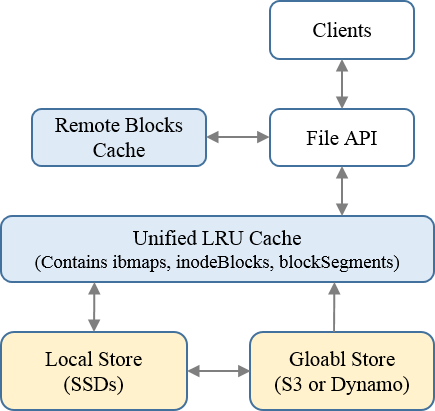
\includegraphics[width=0.4\columnwidth]{{figures/block-diagram.png}}
    \caption{[TBD: caption] Block diagram.}
   \label{fig:block-diagram}
\end{figure}



%\subsection{File Directory} Kawkab filesystem contains a file directory that
%defines the namespace of the system.
%%The file directory keeps track of the existing files in the system and the way
%%to access the files.
%Each file in the system has a unique name and a unique inode number.  The file
%directory is a simple collection of $\langle$ file name, inode number $\rangle$
%pairs that maps a file name to an inode number.  The clients refer to a file
%using the file name whereas the system access the files through the inode
%numbers. 
%
%The file directory is the only structure that keeps the mapping of the file
%names and the inode numbers. Therefore, the file directory is made persistent
%and consistent through a distributed key-value store such as ZooKeeper.
%
%\subtopic{File Namespace:} Kawkab has a flat namespace. Kawkab does not maintain
%directory hierarchies. However, a user can use any file name.
%
%



\section{File Operations}

Kawkab supports the following five file operations:

\subsection{File Open}

A client opens a file to read or to append the file. If the file is opened for
appending, the file is first created if it does not already exist. 

\subtopic{Open-files Table:} Each node keeps track of the open-count for each
file by implementing an open-files table.  The open-files table contains
reference-counts for each file opened for reading or writing on that node.
This table is necessary to correctly implement the file delete operation.
Unlike the standard Unix filesystem, Kawkab does not use file descriptors and
does not return a new file descriptor for each file open request.  Instead, the
file operations are performed using the file's inumber that is returned in a
FileHandle when the file is opened.  The file descriptors are not necessary
because Kawkab is an append-only system and only one file-writer is allowed to
append to the file.


\subtopic{File Creation:} File creation is an atomic operation, which is
performed as follows.
%The node first acquires the file-specific lock that prevents multiple clients
%from creating the same files at the same time.  
The node first assigns an unused inumber from its shard to the new file.  The
node then adds the new filename-to-inode mapping in the file directory.  This
operation succeeds only if the file directory does not already contain the
mapping. This can be achieved, e.g., by using the ZooKeeper's zknode creation
operation.  If the operation succeeds, the node adds an entry in its
\textit{open-files table} and returns successfully to the client.  If the
operation to add the filename-to-inumber mapping in the file directory fails,
the node frees the inumber and returns an error to the client.  


\subsection{File Append}

Kawkab is an append only filesystem -- random writes are not allowed.
Moreover, Kawkab supports single writer and multiple readers at a time.
Initially the node that creates the file becomes the sole writer of the file
and is termed as the file's \textit{primary node}. Only the primary node is
allowed to append to the file~\footnote{ \hl{To discuss: How to prevent multiple file
writers? We need a distributed lock to gain exclusive write
access.}}'\footnote{ \hl{To discuss: How the primary node of a file is changed? How
the file readers are notified updated primary node of the file? We need to
store the primary node information of each file. The node that wants to become
the primary node need to first acquire the distributed lock and then update
primary node information. Finally, the node need to notify the existing file
readers about the updated location of the primary node.}}.
Rest of the nodes can only read the file.

In the file append operation, first the node get the file's inode. The
inode contains the current size and the data index of the file. The
data is then appended at the end of the file. 

\subtopic{Creating New Data Block:}
To append data, first the last data segment of the file is loaded in the cache. 
If the last segment is already full and the segment is the last segment in the 
data block, first a new data block is created.
To create a new block, the node first creates a new block in the local storage.
The new block is created as a new file and the file is filled with random
bytes to reserve the full block space in the local storage.

\subtopic{Appending to Last Segment:}
As data is appended at the end of the file, the cache loads the last data segment
in memory if the segment is not already in the memory.
The data is then appended to the data segment in memory and the data segment
is marked as dirty. After finishing appending data to the segment, the
segment is added in a queue. The queue is continuously emptied using multiple
workers that flush the data segments to the local storage.

\subtopic{Moving Blocks in the Global Storage:}
When all the data segments of the last block are full, the data block is marked
as closed. The closed blocks are then added in another queue that copies
the data block to the global storage. Once the block is copied to the global
storage, the block is then marked as persistent. The persistent blocks
can be deleted from the local storage when the local store need to create
space for more data blocks.


\subtopic{Appending Records:} Kawkab supports two types of append operations. A
file can be appended either using a list of bytes, or using a user defined
records.  In the later case, a record is a fixed size structure that has a user
defined key. Kawkab uses the key to create the data index for the file. For
timestamp based index, it is required that the appended record's key must be
greater than or equal to the last record's key.

Appending records also require updating the data index. In this case, the
data index blocks are also appended and flushed to the local and the
global storage. In Kawkab, the data index blocks are treated in the
same way as the data blocks themselves. Therefore, the index blocks
are cached and persistently stored in the same way as the data blocks.


\subtopic{Updating the Inode:} At the end of the append operation, the file
size and the data index information is updated in the inode. The inode
update marks the inodes block as dirty, which causes the inodes-block
to be flushed to the local storage~\footnote{As an inodes-block consists of
a large number of inodes, we may end up flushing a lot of inodes-blocks. Therefore,
we may need to change the way we store and retrieve inodes}. Inodes-blocks
are periodically updated in the global storage~\footnote{As the global storage
is also likely to be an append only system, it might be better to save inodes-blocks
in a storage that allows random writes, e.g., in a key-value store.}.



\subsection{File Read}

File read operation requires access to the inode and the data segments of the
file. 

\subtopic{Loading Inode:} First the node requires access to the file's inode
that contains the current file size and the data index~\footnote{Note that the
data index is only required if the data is read in a structured way, e.g.,
using record timestamps. If the data is read using the byte offset and the
required data is not located in the last block of the file, the inode access is
not required. It is because the data block ID is a combination of inumber,
block number in the file, and segment number in the block.}.  The node's cache
may need to load the required inodes-block, which contains the file's inode,
from the local or the global storage~\footnote{\hl{To discuss: Do we save the
fetched inodes block in local storage or not? We cannot argue about temporal
locality in the case of inode blocks because each inode represents a different
file and we don't assume any relationship between files.}}.  Inodes-block is
most likely available in the local storage if the node is the primary
node~\footnote{A file's primary node is the node on which the file is opened
for writing. Kawkab allows only one file writer in the system.} of the file.
Otherwise, the inodes-block is loaded from the global store directly into the
cache. In this case, the loaded inodes-block may have the staled file size and
data index. 

If the inode has staled information, the inodes-block can optionally
be fetched from the local storage of the primary node of the file. Currently
the only way to check the freshness of an inode is to read the inodes block
from the file's primary node
\footnote{\hl{To discuss: How do we detect if an inode is staled or not?}}.


%- What if the required data lies beyond the file size in the inodes block?
%  - (1) If the reader is the primary-node of the file
%  - (2) If the reader is the non-primary-node of the file


%The blocks that are loaded from the global storage are not stored in the
%local storage. Instead, the blocks are directly read in the cache. The blocks
%are not saved in the local storage because Kawkab assumes temporal and spatial
%locality of the blocks. Not saving in the local storage saves the
%disk-bandwidth for file-append operations.


\subtopic{Loading Data Segments:}

The inode is used to get the ID of the required data segment. The segment ID is
a combination of inumber, block in the file, and the segment in the block. The
block number can be calculated from the given byte offset or from the file
index if the file is read from the given record index such as timestamp. The
segment ID is then converted to the Base64 key string that represents the
location of the data block in the local storage as well as the global storage.
Moreover, the key string is used to uniquely identify the segment in cache.

If the cache does not already have the required data segments in memory,
the segments are loaded in memory from the local or the global storage.  First
the local storage is queried. If the local storage does not have the required
segments, the complete data block is loaded in memory from the global store.

The data blocks that are downloaded from the global store are placed directly
in the cache instead of saving them in the local store. This is done in order
to take advantage of spatial locality -- it is likely that the complete
block will be read instead of just a few segments in the data block.


If the file reader is not the primary node of the file, it may happen that
the global store has the updated inode but the required data block is not yet
stored in the global store. In that case, the file reader is given an error,
and optionally, the reader can read the required data segment from the local
storage of the primary node of the file. It may also happen that the reader
tries to read from the primary node, whereas in the mean while, the primary node 
transfers the required data block to the global storage and deletes the
block from the local storage. As a result, reading from the primary node
will also fail. Therefore, it is necessary that the file reader
again tries to read from the global store if the file reader is unable to
locate the required segment on the primary node. 


\hl{To discuss: The open-files table should be a distributed table. We need to 
keep the open count globally. The open-files table can also be used to
store the IDs of the file readers that should be notified when the
primary node of the file changes.}


%- Loading cache:
%  - Reading from the local storage
%  - Reading from the global storage
%
%
%- Reading most recent data
%	- Reading from a remote node
%

\subsection{File Close}

%- Deletes file data if the file is marked for deletion

- Updates the open-files table

- The last node that closes the file also deletes the file if the file is
 marked for deletion.


\subsection{File Delete}

- Marks the file as deleted in the open-files table. This prevents further
  file open requests.

- If the open count for the file is greater than one, marks the file
  as deleted. The last one that closes the file deletes the file data.


\section{Filesystem Implementation}

The system is divided in four layers: API, core, main memory, and persistence.
Clients interact with the API layer directly or using an RPC service.  API
provides functions to open, close, read, and write files.


The core layer controls the metadata of the whole system. It mainly consists of
four structures: a file directory, an index node bitmap, index nodes, and data
blocks. Only the data blocks contain the actual data of a file. The other
structures comprise the metadata of the filesystem.


The main memory layer manages the memory usage of a node. 
The memory is divided in a cache and a small buffer for remote segments.
The cache serves as the primary memory resource pool for most of the
in-memory storage of a node. The cache serves as a unified memory
resource pool for most of the operations in the filesystem. The small
buffer is only used to read most recent data segments that are only
available at other nodes in the system.


The persistence layer controls the local and global storage of the system.
A node temporarily saves data on local storage that consists of fast
storage devices such as SSDs or Amazon EBS. The global store persistently
stores all the data.


%\subsection{File Operations}
%
%
%\subsubsection{New File Creation}
%File creation is an atomic operation, which is performed as follows.
%To create a file from a node, the node first acquires the file-specific
%lock that prevents multiple clients from creating the same files at the same time.
%The node then assigns an unused inumber from its shard to the new file.
%In the next step, the node adds the new filename to inode mapping in the
%key-value store. This operation succeeds only if the key-value store
%does not already contains the mapping, e.g., by using the ZooKeeper's
%zknode creation operation. If the operation succeeds, the node adds an entry
%in its \textit{OpenedFiles table} and returns successfully to the client.
%The OpenedFiles table contains reference counts for each file opened for
%reading or writing on that node.
%If the operation to add the filename-to-inumber mapping in the key-value
%store fails, the node frees the inumber and returns an error to the client.
%The lock is released before returning to the client.
%
%%If two different nodes try to create files with the same names, one of the nodes
%%will fail because of atomic data insertion in the key-value store. To create a
%%file, a node first locks its cached 
%
%%It may also happen that two different nodes try to create files with same names.
%%The filesystem will break if two files have same name but different inumbers.
%%To prevent different nodes from creating files with same name, each node
%%first tries to create a file 
%
%%Each file in the system has a unique name and a unique inode number.  The file
%%directory is a simple collection of $\langle$ file name, inode number $\rangle$
%%pairs that maps a file name to an inode number.  The clients refer to a file
%%using the file name whereas the system access the files through the inode
%%numbers.
%%
%%The file directory is the only structure that keeps the mapping of the file
%%names and the inode numbers. Therefore, the file directory is made persistent
%%and consistent through a distributed key-value store such as ZooKeeper.
%%
%
%
%%The system is designed such that the files are stored in a very large linear
%%storage space. The files have a unique name, which is stored in a file
%%directory.  The filesystem does not support directory structures. The file
%%directory instead contains filename to file ID mappings. File ID is a globally
%%unique, i.e., filesystem wide, 64-bit number assigned to the files.

\subsection{File Read Operation}

\subsection{File Append Operation}

\subsection{File Delete Operation}




%\section{Persistence Layer}
%\hl{Note: This section is incomplete.}
%
%The persistence layer in Kawkab keeps track of the location of each file in the system.
%All the blocks are stored and retrieved from the persistence layer using the UUIDs
%of the blocks.
%
%The persistence layer has a caching sub-module. The caching module acts as an
%LRU cache and controls the memory of one machine.
%
%
%\subsection{Block Metadata} In order to achieve faster data access, each block
%has an associated metadata that is stored along with the block's UUID. The
%metadata includes: first append time, last append time, and the additional
%data boundaries that allow fine grained indexing within a data block.
%


%\subsection{Local Store}


%\subsection{Global Store}

\begin{figure}[t]
    \centering
    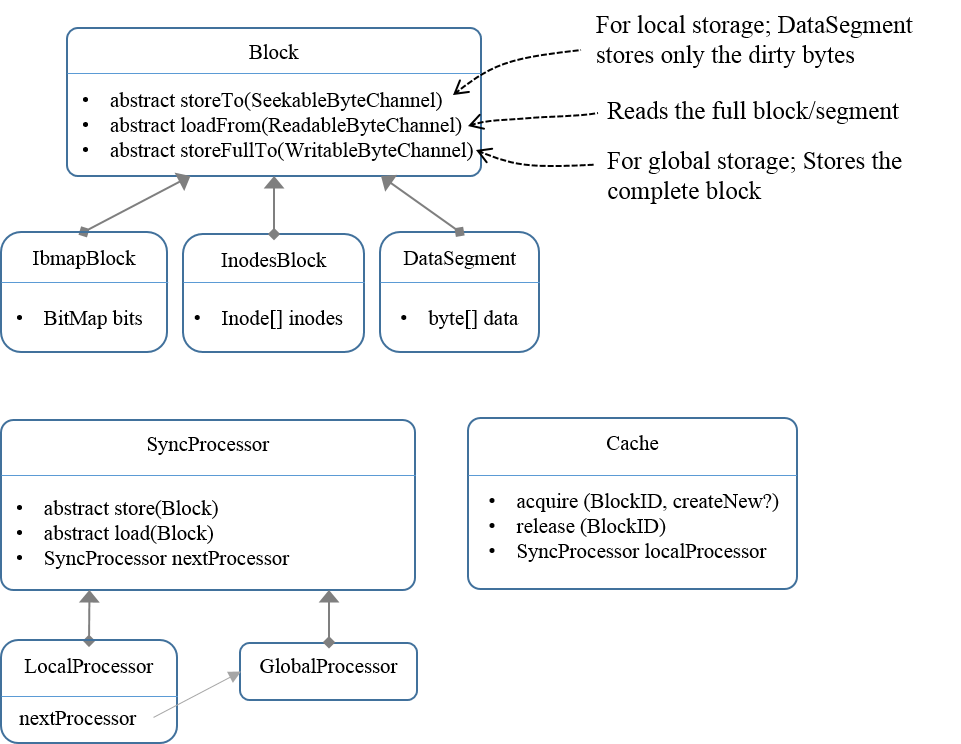
\includegraphics[width=0.9\columnwidth]{{figures/class-diagrams.png}}
    \caption{Class diagrams.}
   \label{fig:data-structures}
\end{figure}



%\begin{figure}[t]
%    \centering
%    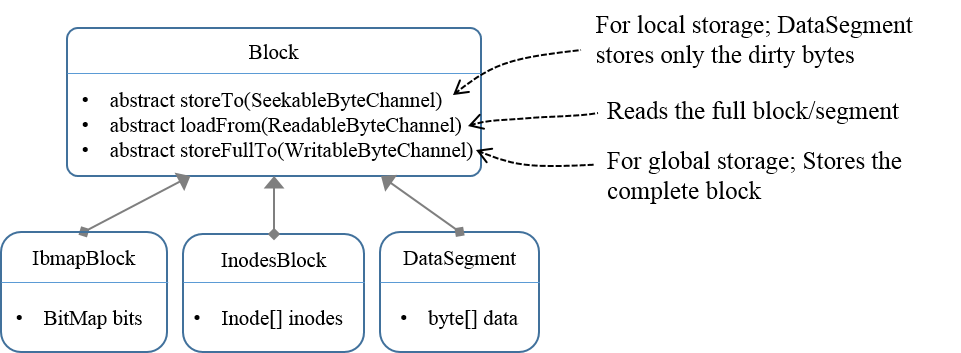
\includegraphics[width=0.8\columnwidth]{{figures/class-diagram-blocks.png}}
%    \caption{[TBD: caption] Class diagram of the blocks.}
%   \label{fig:data-structures}
%\end{figure}
%
%
%\begin{figure}[t]
%    \centering
%    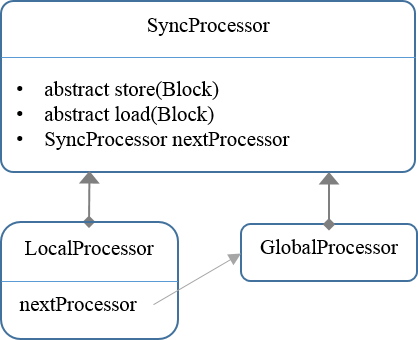
\includegraphics[width=0.4\columnwidth]{{figures/class-diagram-syncprocs.png}}
%    \caption{[TBD: caption] Class diagram of the sync-processors.}
%   \label{fig:data-structures}
%\end{figure}


\subsection{Atomic Appends and Reading Unfinished Block}

\section{Extensible Indexing}

\hl{Note: This section is incomplete.}

Kawkab is an append-only system. Each append is performed at the end of the file.
However, a file can be read from any location. When a client opens a file,
it is returned a FileHandle. The FileHandle contains a read pointer that indicates
the current position in the file from where the data will be read. The read
pointer can be moved to any position in the file using any of the following
ways: 

\begin{enumerate}
  \item Move to an absolute byte offset in the file.
  \item Give a timestamp T:
  \begin{itemize}
    \item Move to the first byte of the closest block that has the append time equal to
          or \textit{before} T.
    \item Move to the first byte of the closest block that has the append time equal to
          or \textit{after} T.
  \end{itemize}
\end{enumerate}

In order to find the data block that contains the given byte or timestamp, Kawkab
performs binary search over the index in the inode.

Todo:

\begin{itemize}
  \item Indexing within a block
  \item Time range queries
\end{itemize}

%  - How data is indexed
% - How data is retrieved given a byte offset
 % - How data is retrieved given a timestamp



\section{Distributed Design of Kawkab}

\hl{Todo: Need to be revised.}

\subsection{Distributed Metadata and Namespace}

In Kawkab, only the filesystem namespace (file directory) and other metadata
(ibmaps and inodes) are concurrently updated across the nodes. Data blocks are
not updated concurrently. Therefore, Kawkab uses a distributed key-value store
to safely and consistently store only the namespace. The other metadata
is partitioned across the nodes.

\subtopic{Key-Value Store Consistency Requirements:} The basic requirement for
metadata consistency is that all of the nodes in Kawkab observe the same
sequence of updates to the file directory, the ibmaps, and the inode blocks.  
%As Kawkab allows only one file writer at a time, the indirect blocks, which
%contains the UUIDs of the data blocks and indirect blocks, do need to be made
%consistent across the nodes.
Therefore, the key-value store is required to provide at least sequential
consistency.
%The keys are file IDs and the values are the inode numbers in the key-value
%store.
We propose to use ZooKeeper because it allows conditional creation of the
nodes: an error is generated if a client tries to create an already existing
node. Moreover, ZooKeeper allows the clients to subscribe for notifications
when a node is updated.  These features can be used to maintain consistency
of the file directory across all the nodes in Kawkab.


\subsubsection{Data Blocks and Indirect Blocks} Data blocks are stored locally
on SSDs and remotely in the cloud storage such as EBS and S3. Data blocks are
not replicated to the storage of other nodes.

\subtopic{File Appends:} The file writer appends data in memory. The data
blocks are then flushed to the local SSD asynchronously for faster file write
operations. When a data block is closed, it is copied to the cloud storage.

\subtopic{File Reads:} Remote nodes read data blocks directly from the cache,
or from the cloud storage (EBS/S3) if the data blocks are not in cache.  If a
data block does not exist in the remote storage, e.g., if it is the last block
in file or the block is not yet replicated in the cloud storage, the reader
node fetches the desired block from the primary node of the file where the file
writer is located. The fetched data block is then kept in the LRU cache.

\subtopic{Indirect Blocks:} Indirect blocks, which contain the UUIDs of other
indirect blocks or data blocks, are treated the same as the data blocks.
%Indirect blocks contains UUIDs of data blocks and other indirect blocks. 
Only the file writer can update a data block or an indirect block. Therefore,
indirect blocks are stored and accessed the same was as the data blocks.


\subsubsection{Namespace Replication and Consistency}
Kawkab uses ZooKeeper to keep the namespace consistent. All the file
directory information, which consists of mappings from file IDs to the
inumbers (inode number), in ZooKeeper. ZooKeeper is a good candidate
for the namespace because the frequency of the creation of new files is low
and the higher latency for the file create operation is acceptable.

When a node creates a new file, it adds a zknode in ZooKeeper on the path
\texttt{kawkab/files/fileID} and with the node-value of the inumber assigned to
the file. If the node creation fails due to an already existing zknode with
the same path, it implies that another node has already created the file with the same
file ID. Therefore, the file opening for writing is failed. However, the file can be
opened for file reads in this situation. In this way, all the nodes view
the same file directory across the system.

The file directory is kept in cache on each node for faster file read and write
operations. Moreover, the file directory is periodically updated to reflect the
recent changes in the directory. This can be achieved by each node subscribing
to the zknode update events for \texttt{kawkab/files}.

For the file open requests in the read-only mode, first the file directory in
the cache is used to get the inumber of the file. If the file is not found in
the cache, the node reads the file from the ZooKeeper and updates the file
directory if the file is found.



\subsubsection{Ibmap and Inode-blocks Partitioning} Kawkab partitions the ibmap
and the inode blocks space across the nodes. Each node is assigned a specific
number of ibmap-blocks and the corresponding inode blocks.
%For example, N ibmap blocks and the corresponding inode blocks are assigned to
%each node. 
The blocks are assigned in a sequential order. The partitioning ensures that
each node uses a unique inumber for the new files without any synchronization
overhead.

\subtopic{Persistence:} Each node persistently stores its Ibmap blocks and the
inode blocks in its local storage as well as the remote storage. The blocks are
periodically flushed to these storage to reduce the memory and the network usage.

\subtopic{Inode Updates Across Nodes:} Inodes are frequently updated as an inode is
updated after each file append operation to reflect the changes in the file
size and the other metadata (e.g., last modified time).  Therefore, inodes need
to be made consistent across all the readers of the file.

Kawkab uses a simple publish-subscribe system to propagate the inodes' updates
across the nodes where the file-readers are located. Each node with
at least one active reader subscribes to the inode updates on the primary node
of the file, i.e., where the file writer is located. The file writer 
asynchronously publishes the inodes to all the subscribers. In this way,
the staleness of the inodes is reduced on the file readers.


\subtopic{Inodes Location from Inumbers:} It may happen that a node opens a
file for reading while the file has been created by another node. As the
location of an inode cannot be inferred from an inumber, Kawkab also stores the
mapping of the inumber range to the node location in ZooKeeper.  For example,
if $x$ inodes are assigned to each node, Kawkab stores the mappings $\langle x
\to \mathrm{node1} \rangle$, $\langle 2x \to \mathrm{node2} \rangle, \ldots$,
in the ZooKeeper, which implies that the inodes from $x$ to $2x-1$ are stored
in the node with ID $\mathrm{node1}$. As this information is static and do not
change frequently, all the nodes cache this information during bootstrap. If
the information is updated due to node failures, all the nodes are updated to
reflect the changes in their cache.



\subsection{Scalability}

\subsection{Fault-tolerance}

\subsection{Consistency Guarantees}

\subsection{Metadata and Data Journaling}

%\subtopic{Creating a New File:}
%\begin{itemize}
%  \item Get inumber \texttt{inum} from the ibmap
%  \item Execute a multi-operation transaction in ZooKeeper:
%  \begin{itemize}
%    \item Create a persistent node with path \texttt{kawkab/inodes/inum}.
%    \item Create a persistent node with path \texttt{kawkab/files/fileID} and the value equals to \texttt{inum}.
%  \end{itemize}
%  \item If the previous transaction succeeds, update the local file directory and the ibmap.
%  \item If the transaction fails, it is because either (1) The inode is already consumed, or (2) the file already
%        exists. If the file already exists, then the file creation operation returns with FileExists error. If the
%        inode is already consumed, 
%\end{itemize}


%\subsection{Distributed Namespace:}
%Kawkab partitions the namespace across all the nodes. Each node has a dedicated
%namespace, and each node creates new files in its own namespace. The metadata
%belonging to each namespace -- files directory, ibmaps, and inode blocks --
%are kept consistent across all the nodes.

%\section{File Read and Write Operations}

\section{Workload}

\subsection{File Access Patterns}

\subtopic{File Writes:} Kawkab allows only one writer at a time to
write the file. The first client that opens the file becomes the distinguished
writer of the file. Only the distinguished writer is then allowed to append to
the file. Moreover, the node where the client is located becomes the primary
node of the file.  The other nodes may fetch recent appends from the primary
node when the data is not replicated in the cloud storage (S3/EBS).

If an existing writer fails, another client can become the distinguished writer
by successfully opening the file for writing. If the writer closes the file,
another writer can open the file and become the distinguished
writer\footnote{In the Smash's use case, files are never closed.}. However,
Kawkab allows only one file writer at a time.

Each append request consists of small number of bytes, e.g., less than 100 bytes.

\subtopic{File Reads:}
Kawkab allows multiple readers to read at the same time. If the data block
is not located locally in the system, the data block is fetched from S3/EBS if
it is available. If the data block is not available in S3/EBS, the data block
is fetched from the node where the file-writer is located.

Todo: Data access frequency and size, number of readers per node, number of
nodes where readers are located $\ldots$.




\section{Related Work}

\begin{easylist}[itemize]

 # Comparison with Alluxio

 # Comparison with Succinct

 # Comparison with HDFS and similar systems

\end{easylist}



\end{document}
